\documentclass[12pt, a4paper]{book}
\usepackage[utf8]{inputenc}
\usepackage{fullpage}
\usepackage{amsmath}
\usepackage{amssymb}
\usepackage{graphicx}
\usepackage{mathtools}
\usepackage[comma,authoryear]{natbib}
\usepackage{listings}
\usepackage{color}
\usepackage{wrapfig}

\definecolor{dkgreen}{rgb}{0,0.6,0}
\definecolor{gray}{rgb}{0.5,0.5,0.5}
\definecolor{mauve}{rgb}{0.58,0,0.82}

\lstset{frame=tb,
  language=R,
  aboveskip=3mm,
  belowskip=3mm,
  showstringspaces=false,
  columns=flexible,
  basicstyle={\small\ttfamily},
  numbers=none,
  numberstyle=\tiny\color{gray},
  keywordstyle=\color{blue},
  commentstyle=\color{dkgreen},
  stringstyle=\color{mauve},
  breaklines=true,
  breakatwhitespace=true,
  tabsize=3
}
\linespread{1.3}
\graphicspath{{./}}
\title{Big Data Energy 2020 TAMIDS Competition}
\author{Johnathan Lo \& Isaac Ke}
\date{3/28/20}

\newcommand{\R}{\mathbb{R}}
\newcommand{\Z}{\mathbb{Z}}
\newcommand{\Lagr}{\mathcal{L}}
\newcommand\tab[1][1cm]{\hspace*{#1}}

\begin{document}
\maketitle
\tableofcontents
\chapter{Introduction}
\tab Reliable transportation supports a strong economy by facilitating the rapid and timely exchange of goods and services and bolstering tourism revenue. In the US, the transportation industry accounts for XXX billion dollars per year, which is XXX\% of GDP [cite]. Of that economic product, XXX\% is accounted for by the airline industry [cite]. A key metric for evaluating the efficiency of airline industry production is flight delay time. In 2018, flight delays led to an economic loss of XXX billion dollars[cite]. For individual companies, delays can influence consumer choice, and for the industry itself, unmitigated delays can impel consumers to switch to substitute goods, such as automotive or rail-based transport. \\
\tab Therefore, a major goal of this project is to analyze flight delays and diagnose areas for improvement. We intend to create models using publicly available data that can accurately predict future delays. In doing so, we can hopefully uncover significant and controllable covariates that can help guide airline companies to reduce flight delays. 

\chapter{Executive Summary}
	\section{Problem and approach}
	\section{Data preprocessing}
	\section{Exploratory analysis}
	\section{Model formulation}
	\section{Model selection}
	\section{Applications and conclusions}
	
\chapter{Motivation, data description, and software}
	\section{Motivation}
	\tab As stated in the introduction, flight delays can have a wide-ranging effect on the economy. Most airline companies have already done everything in their power to mitigate and reduce delays. We are interested in finding whether delays can be further mitigated, and whether those variables can be controlled by airline companies. To the extent that some delays are unavoidable or difficult to predict, we are also interested in devising methods to minimize the impact of those delays, whether by reducing the number of passengers affected, offering alternate routes to affected passengers, or discounting tickets. Overall, for the benefit of airline companies, consumers, and society-at-large, we should minimize flight delays, or the impact thereof. 
	\section{Data collection}
	\tab Our data was provided to us as csv files by the competition organizers. The primary dataset was composed of over 10,000,000 observations of 50 variables. Each observation was a distinct flight that occurred between 1/1/2018 and XX/XX/2019, and the 70 covariates included origin, destination, quarter, arrival delay, departure delay, distance, and many more variables pertaining to each flight. An auxiliary dataset included pricing data given for each route, by quarter. \\
	\tab In addition to the data provided to us by the competition organizers, we also sought out additional data to enhance our dataset. We obtained geographic coordinates for each airport from XXXXX [cite], and weather data from NOAA databases through the NCDC API [cite]. The geographic coordinates are given in decimal format, and our weather data describes meteorological events near the origin and destination of each flight. Importantly, data \textit{along} the flight path was not obtained, due to time constraints and complexity. A full list of covariates along with brief descriptions can be found in \underline{Supplementary Table 1}. 
	\section{Software}
	\tab All analyses were performed in R v3.6.3 [cite]. Packages used include, but are not limited to, \textit{ggplot2}, \textit{dplyr}, \textit{caret}, \textit{rnoaa}, and \textit{Isaac put stuff here}. Individual datasets were loaded as \textit{data.frame} objects and combined using \textit{merge}. The final dataset can be found as a csv file in \underline{Supplementary Data 1}. 
	
\chapter{Exploratory data analysis}

	\section{Data wrangling}
	
	\tab Our dataset was drawn from 4 different sources - flight delays and fare data, provided to us by the competition organizers, geographic coordinates from XXXXX, and weather data from NOAA. Flight delays and geographic coordinates were combined by merging on common  origin and destination names. The resulting dataframe was then combined with fare data by common routes, year, and quarter. Adding weather data was more challenging in that the observations relate information collected by weather stations, and not the airports themselves. Thus, weather station coordinates were cross referenced with airport coordinates to find the closest active weather station to each airport. Due to this constraint, 10 airports, corresponding to 99980 observations, were dropped, due to the lack of NOAA weather stations nearby. Weather data was then merged with the rest of the data on common dates and airports, with separate variables for weather at origin and weather at destination.  The final dataset containing all 4 sets of information is what will be referenced in this paper hereafter.\\
	
	\tab The data contained a number of variables with numerical values but that could be interpreted either as quantitative or categorical variables. Using substantive knowledge, a number of numeric variables were converted to factors, including day of week, month, quarter, and route number. Additionally, our data contained many missing values. Where applicable, for categorical variables, these values were replaced by adding an additional factor level \textit{Unk}. For quantitative variables, missing values were replaced with either 0, or observations were removed, based on substantive knowledge of the variable characteristics. Finally, the flight delay data somewhat bewilderingly assigned canceled flights a delay time of 0. Canceled flights were removed from the dataset and analyzed separately.  In all, the final dataset consisted of 10614150 observations of 100 variables. 
	
	\section{Distribution of flight delays}
	
	\tab A histogram of all arrival delays is shown in \underline{Fig 1}. Clearly, the data is strongly right-skewed. To correct the skewness, a cube-root transformation was performed, but subsequent Shapiro-Wilk test provided strong evidence against normality for this transformation, so it was abandoned. To heuristically assess dependence between covariates and response, we examined various conditional distributions.\\
	\begin{wrapfigure}{l}{0.45\textwidth}
	\centering
	 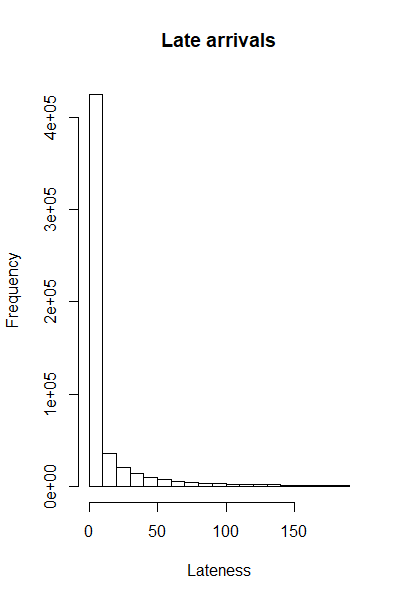
\includegraphics[width = .45 \textwidth]{../figures/LateArrivalsHistogram}
	 \caption{Fig 1 - Histogram of arrival time for all observations in the dataset}
	 \end{wrapfigure}
	 
		\subsection{Geographic distribution of flight delays}
		
			\tab The distribution of flight delays across the geographic United States is shown in \underline{Fig 2}. As we can see, XXXXX XXXXX XXXXX XXXXX XXXXX XXXXX XXXXX XXXXX XXXXX XXXXX XXXXX XXXXX XXXXX XXXXX XXXXX, XXXXX XXXXX XXXXX XXXXX XXXXX XXXXX XXXXX XXXXX XXXXX XXXXX XXXXX XXXXX XXXXX XXXXX XXXXX. XXXXX XXXXX XXXXX XXXXX XXXXX XXXXX XXXXX XXXXX XXXXX XXXXX XXXXX XXXXX XXXXX XXXXX XXXXX. XXXXX XXXXX XXXXX XXXXX XXXXX XXXXX XXXXX XXXXX XXXXX XXXXX XXXXX XXXXX XXXXX XXXXX XXXXX.\\
			\begin{wrapfigure}{r}{0.45\textwidth}
			\centering
	 		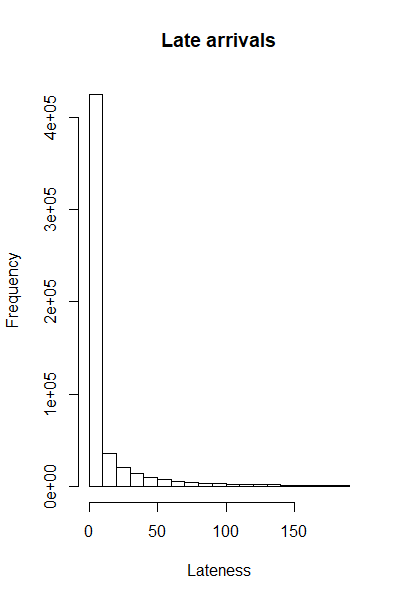
\includegraphics[width = .45 \textwidth]{../figures/LateArrivalsHistogram}
	 		\caption{Fig 2 - Figures showing the geographic distribution of flight delays by delay length and airport usage}
	 		\end{wrapfigure}
	 		
		\subsection{Temporal distribution of flight delays}
		
			\tab In \underline{Fig 3}, we demonstrate the distribution of flight delays by time of day, day of week, month, and quarter.  As we can see, XXXXX XXXXX XXXXX XXXXX XXXXX XXXXX XXXXX XXXXX XXXXX XXXXX XXXXX XXXXX XXXXX XXXXX XXXXX, XXXXX XXXXX XXXXX XXXXX XXXXX XXXXX XXXXX XXXXX XXXXX XXXXX XXXXX XXXXX XXXXX XXXXX XXXXX. XXXXX XXXXX XXXXX XXXXX XXXXX XXXXX XXXXX XXXXX XXXXX XXXXX XXXXX XXXXX XXXXX XXXXX XXXXX. XXXXX XXXXX XXXXX XXXXX XXXXX XXXXX XXXXX XXXXX XXXXX XXXXX XXXXX XXXXX XXXXX XXXXX XXXXX.
			\begin{wrapfigure}{l}{0.45\textwidth}
			\centering
	 		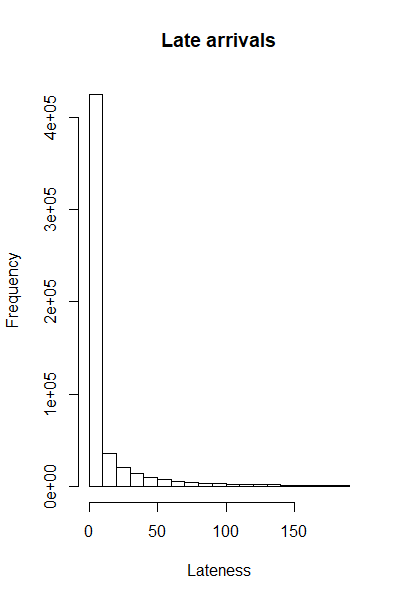
\includegraphics[width = .45 \textwidth]{../figures/LateArrivalsHistogram}
	 		\caption{Fig 3 - Histograms of ARR DELAY by time of day, day of week, month, and quarter}
	 		\end{wrapfigure}
	 		
		\subsection{Weather-based distribution of flight delays}
		
			\tab Our weather data provided us primarily with data on precipitation and temperature. Other events, such as heavy fog and ice, were observed, but sparse. We show scatterplots of flight delays by precipitation and temperature in \underline{Fig 4}. In \underline{Fig 5}, histograms of flight delays for some unusual weather events are given. XXXXX XXXXX XXXXX XXXXX XXXXX XXXXX XXXXX XXXXX XXXXX XXXXX XXXXX XXXXX XXXXX XXXXX XXXXX, XXXXX XXXXX XXXXX XXXXX XXXXX XXXXX XXXXX XXXXX XXXXX XXXXX XXXXX XXXXX XXXXX XXXXX XXXXX. XXXXX XXXXX XXXXX XXXXX XXXXX XXXXX XXXXX XXXXX XXXXX XXXXX XXXXX XXXXX XXXXX XXXXX XXXXX. XXXXX XXXXX XXXXX XXXXX XXXXX XXXXX XXXXX XXXXX XXXXX XXXXX XXXXX XXXXX XXXXX XXXXX XXXXX.
			\begin{figure}[h]
	 		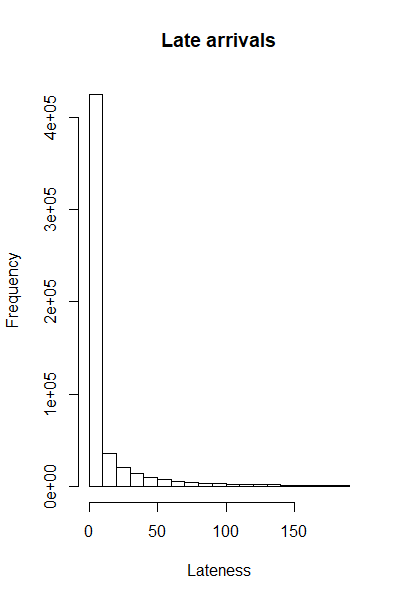
\includegraphics[width = .75 \textwidth]{../figures/LateArrivalsHistogram}
	 		\caption{Fig 4 - scatterplots of ARR DELAY by precipitation and temperature}
	 		\end{figure}
	 		\begin{figure}[h]
	 		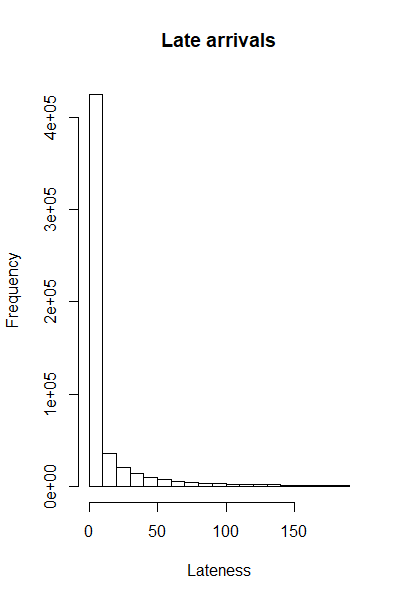
\includegraphics[width = .75 \textwidth]{../figures/LateArrivalsHistogram}
	 		\caption{Fig 5 - histograms of ARR DELAY for each unusual weather event}
	 		\end{figure}
		\subsection{Carrier-based distribution of flight delays}
			
			\tab For each of the 19 carriers, flight delays was plotted. Histograms for each are given in \underline{Fig 6}. We also hypothesized that there might also be differences in flight delays between different carriers. A one-way ANOVA was conducted, and p-values corrected using Tukey's HSD, shown in \underline{Fig 7}.
			\begin{figure}[h]
	 		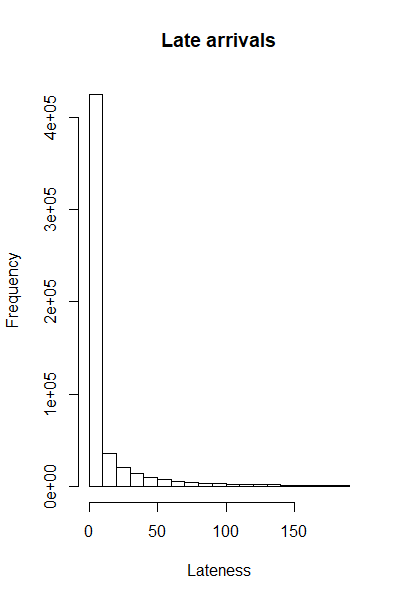
\includegraphics[width = 1 \textwidth]{../figures/LateArrivalsHistogram}
	 		\caption{Fig 6 - Histograms for the airlines}
	 		\end{figure}
	 		\begin{figure}[h]
	 		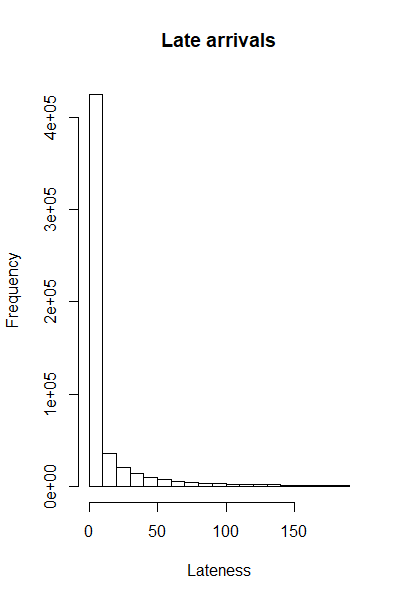
\includegraphics[width = 1 \textwidth]{../figures/LateArrivalsHistogram}
	 		\caption{Fig 7 - airline ANOVA}
	 		\end{figure}

		\subsection{Airport-based distribution of flight delays}
			
			\tab We were also interesting in detecting if individual airports showed differences in flight delays, shown in \underline{Fig 8}. 
			\begin{figure}[h]
	 		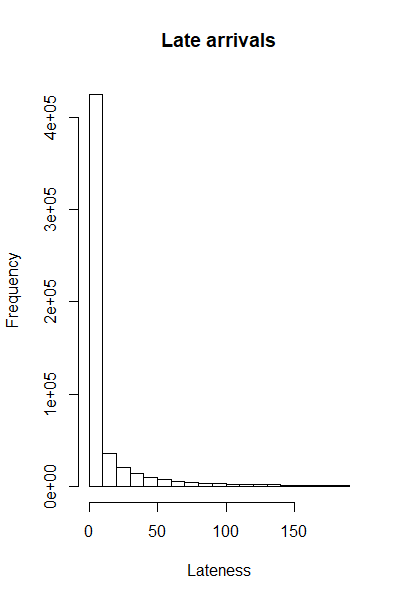
\includegraphics[width = 1 \textwidth]{../figures/LateArrivalsHistogram}
	 		\caption{Fig 8 - Airport histograms}
	 		\end{figure}
	 		
\chapter{Model formulation}
\chapter{Model selection}
\chapter{Forecasting Flight Delays for 2019 Q3}
\chapter{Business recommendations}
\chapter{Closing thoughts}
\chapter{Appendix}
	\section{References}
	\section{Additional figures, tables, and data}
\pagebreak

\bibliographystyle{natdin}
\nocite{*}
\bibliography{sources}
\end{document}